\documentclass[UTF8,a4paper,12pt,fontset=none]{ctexart}
\usepackage[margin=2.5cm]{geometry}
\usepackage{amsmath,amssymb,amsthm}
\usepackage{graphicx}
\usepackage{booktabs}
\usepackage{longtable}
\usepackage{array}
\usepackage{float}
\usepackage{caption}
\usepackage{xcolor}
\usepackage{hyperref}
\usepackage{setspace}
\usepackage{listings}
\usepackage{enumitem}
\usepackage{subcaption}
\setCJKmainfont{Noto Serif CJK SC}
\setCJKsansfont{Noto Sans CJK SC}
\setCJKmonofont{Noto Sans Mono CJK SC}
\setstretch{1.32}
\setlength{\parskip}{0.35em}
\setlist{itemsep=0.15em, topsep=0.25em}
\emergencystretch=2em
\ctexset{
    section = {name = {}, number = \arabic{section}, aftername = \quad},
    subsection = {name = {}, number = \arabic{section}.\arabic{subsection}, aftername = \quad}
}
\hypersetup{colorlinks=true,linkcolor=blue,citecolor=blue,urlcolor=blue}
\lstset{basicstyle=\ttfamily\small,breaklines=true,frame=single,columns=fullflexible,keepspaces=true}
\graphicspath{{../../}{../../report_assets/Homework2/figures/}}

\title{最优化作业2：算法实现、理论推导与 Burgers PINN 参数轨迹分析}
\author{}
\date{2026年5月}

\begin{document}
\maketitle
\tableofcontents
\newpage

\section{摘要}

本报告围绕作业2中给出的 17 个问题，统一完成了算法实现、数值实验、理论推导与文献调研。代码部分以 Python 为主，围绕一套轻量级优化框架实现了精确一维搜索、不精确一维搜索、Fletcher--Reeves 共轭梯度法、DFP、BFGS，以及深度学习中常见的一阶改进优化器；理论部分则对次微分、带噪声随机梯度、梯度下降收敛性、共轭函数和对偶性等问题进行了系统整理；扩展实验部分利用仓库中已有的 Burgers PINN 训练结果，对随机初始化与参数低维轨迹现象进行了分析。

数值结果表明：在题目给定的二次问题上，FR 共轭梯度、DFP 和 BFGS 都能在 2 步内恢复解析解；在题目给定的两道一维二次问题上，黄金分割法、斐波那契法、二分法和 Shubert--Piyavskii 方法均达到了题目要求的区间精度；在 Rosenbrock 方向搜索问题上，Goldstein、Armijo、Wolfe--Powell 和强 Wolfe 规则都给出了可接受步长，但接受的步长长度和曲率条件差异明显。对深度学习优化器的扩展实验显示，在二维二次问题上，自适应方法对病态曲率更敏感，而在步长经过调节的简单确定性问题上，普通 SGD 仍可能取得最优结果。

Burgers PINN 的额外分析进一步表明：不同随机初始化下训练得到的最终参数向量在参数空间中相距很远，参数余弦相似度接近 0，但对应网络的预测差异却很小；若将多种方法、多个随机种子以及不同训练时刻的参数向量联合做 PCA，前两个主成分解释了 63.29\% 的方差，前三个主成分解释了 77.27\% 的方差，说明训练轨迹确实呈现出显著的低维结构，但这一结构并非完全集中在二维平面中。对 Krylov 子空间方法的示例实验显示：在对称正定三对角矩阵上，CG 明显快于 GMRES；而在非对称三对角矩阵上，GMRES 仍然稳定收敛，说明其适用范围更广。

\section{任务概览与实现框架}

本次作业的实现遵循“同一抽象服务多道题目”的原则，而不是为每一道题分别编写独立脚本。代码与报告资产组织如下：

\begin{table}[H]
\centering
\scriptsize
\resizebox{\textwidth}{!}{%
\begin{tabular}{lll}
\toprule
类型 & 路径 & 说明 \\
\midrule
算法入口 & \texttt{tools/Homework2/run\_core\_tasks.py} & Q1--Q3、Q5--Q7 的核心算法实验 \\
报告分析入口 & \texttt{tools/Homework2/run\_report\_tasks.py} & Q9、Q13、Q14、Q16 的图表与摘要生成 \\
算法模块 & \texttt{tools/Homework2/src/} & 问题定义、线搜索、拟牛顿、深度学习一阶优化器 \\
结果资产 & \texttt{report\_assets/Homework2/} & figures、tables、raw 三类产物 \\
LaTeX 报告 & \texttt{Latex/Homework2/homework2\_report.tex} & 本报告主文件 \\
\bottomrule
\end{tabular}
}
\end{table}

实验运行主要依赖现有的 \texttt{config-pinn} conda 环境，其中已经包含 \texttt{numpy}、\texttt{scipy}、\texttt{matplotlib} 和 \texttt{torch}。在实现层面，精确搜索与不精确搜索被放在同一线搜索模块中，DFP、BFGS 和 FR 共轭梯度则共享同一套历史记录格式和结果导出接口。这种组织方式使得 Q1、Q5、Q6、Q7 之间可以直接共享同一套方向更新与步长搜索接口；Q13 中的 SGD、Momentum、RMSprop 和 Adam 则被统一到一个独立的一阶优化器模块中，用于说明“深度学习优化器”与经典数值优化之间的关系。

\section{一维搜索、共轭梯度与拟牛顿实验}

本节对应题目中的 Q1、Q2、Q3、Q5、Q6 和 Q7，重点回答“如何实现算法”和“实际迭代行为如何”。

\subsection{题目二：精确一维搜索方法比较}

Q2 要求分别用黄金分割法、斐波那契法、二分法与 Shubert--Piyavskii 方法求解两道一维二次问题。由于两道题都是严格凸二次函数，解析极小点分别为
\[
x_{\mathrm{Q2(a)}}^*=0.25,\qquad x_{\mathrm{Q2(b)}}^*=3.6.
\]
题目给出的不是函数值精度，而是区间精度，因此评价重点应放在“最终搜索区间是否足够短”和“极小点估计是否落在可接受误差范围内”。

\begin{table}[H]
\centering
\scriptsize
\resizebox{\textwidth}{!}{%
\begin{tabular}{llrrrr}
\toprule
问题 & 方法 & 迭代次数 & 近似极小点 & 极小点误差 & 函数值误差 \\
\midrule
Q2(a) & Golden section & 8 & 0.257354 & 0.007354 & $1.0817\times10^{-4}$ \\
Q2(a) & Fibonacci & 8 & 0.218182 & 0.031818 & $2.0248\times10^{-3}$ \\
Q2(a) & Bisection & 3 & 0.250000 & 0 & 0 \\
Q2(a) & Shubert--Piyavskii & 10 & 0.265702 & 0.015702 & $4.9311\times10^{-4}$ \\
Q2(b) & Golden section & 12 & 3.608631 & 0.008631 & $2.2346\times10^{-4}$ \\
Q2(b) & Fibonacci & 13 & 3.586066 & 0.013934 & $5.8250\times10^{-4}$ \\
Q2(b) & Bisection & 8 & 3.613281 & 0.013281 & $5.2917\times10^{-4}$ \\
Q2(b) & Shubert--Piyavskii & 44 & 3.642052 & 0.042052 & $5.3050\times10^{-3}$ \\
\bottomrule
\end{tabular}
}
\caption{Q2 精确一维搜索结果摘要}
\label{tab:q2-summary}
\end{table}

从结果可以看出，二分法在这两道题上最准确，其原因并不是二分法本身“总优于”其他方法，而是因为这里额外利用了导数符号信息。黄金分割法和斐波那契法只依赖函数值比较，因此在给定区间精度下得到的近似点略粗，但仍满足题目要求。Shubert--Piyavskii 方法需要 Lipschitz 常数上界，理论上适用于更一般的 Lipschitz 优化问题，在当前简单二次问题上并不占优势，因此迭代次数最高。
严格来说，表 \ref{tab:q2-summary} 中不同方法可利用的信息并不完全相同：二分法使用了导数符号，而黄金分割法、斐波那契法和 Shubert--Piyavskii 方法仅使用函数值。因此，这里的结论应理解为“在题目允许使用导数信息时，二分法最节省迭代”；若只允许函数值 oracle，则更公平的比较应在黄金分割法、斐波那契法与 Shubert--Piyavskii 之间进行。另一个需要说明的细节是，Shubert--Piyavskii 方法对 Lipschitz 常数上界较为敏感；本报告使用的是保守上界，因此它的区间收缩速度偏慢，这一结果更接近“稳健但保守”的实现状态，而不是该方法的最佳可能表现。

\subsection{题目三：不精确一维搜索在 Rosenbrock 方向子问题上的表现}

Q3 固定 Rosenbrock 函数
\[
f(x)=100(x_2-x_1^2)^2+(1-x_1)^2,
\]
并令初始点为 $x^{(0)}=(-1,1)^T$、搜索方向为 $d=(1,1)^T$，要求比较 Goldstein、Armijo、Wolfe--Powell 以及改进规则。这里研究的不是二维优化全过程，而是单条方向上的步长选择问题，即最小化
\[
\phi(\lambda)=f(x^{(0)}+\lambda d).
\]

\begin{table}[H]
\centering
\scriptsize
\resizebox{\textwidth}{!}{%
\begin{tabular}{lrrrr}
\toprule
方法 & 迭代次数 & 接受步长 $\alpha$ & 新点函数值 & 新点方向导数 \\
\midrule
Goldstein & 10 & 0.001953125 & 3.995620 & -0.487332 \\
Armijo & 9 & 0.00390625 & 3.998087 & 3.011621 \\
Wolfe--Powell & 9 & 0.00390625 & 3.998087 & 3.011621 \\
Strong Wolfe & 9 & 0.00390625 & 3.998087 & 3.011621 \\
\bottomrule
\end{tabular}
}
\caption{Q3 不精确一维搜索结果摘要}
\end{table}

该结果说明，不精确线搜索的核心并不是“逼近精确极小步长”，而是尽快找到一个满足下降条件和曲率条件的可接受步长。Goldstein 条件给出的步长更保守，因此接受的 $\alpha$ 更小；Armijo 只要求充分下降，因而容易接受较大步长；Wolfe--Powell 与强 Wolfe 规则额外控制曲率，给出的结果与 Armijo 接近，但解释上更强调曲率信息而不是单纯下降量。
需要特别说明的是，表中的“新点方向导数”在 Armijo、Wolfe--Powell 和强 Wolfe 情形下为正，这并不意味着算法出错。原因在于：Armijo 条件只要求函数值有足够下降，并不要求新点的一维导数仍然为负；而 Wolfe 类条件要求的是曲率条件，允许搜索步长越过一维极小点，只要新的导数满足规定的不等式即可。换言之，对不精确线搜索而言，“接受步长”与“命中一维极小点”本来就是两个不同目标。

\subsection{题目一、五、六、七：FR 共轭梯度、DFP 与 BFGS}

Q1、Q5、Q6、Q7 都是二维二次问题，因此是检验拟牛顿法和共轭梯度法实现是否正确的理想对象。本文对这些题统一采用精确一维搜索，其中方向搜索使用一维导数二分法完成。解析解分别为：Q1 的最优点为 $(-1,1.5)^T$，Q5 的最优点为 $(0,0)^T$，Q6 的最优点为 $(2,1)^T$，Q7 的最优点为 $(8,6)^T$。

\begin{table}[H]
\centering
\scriptsize
\resizebox{\textwidth}{!}{%
\begin{tabular}{llrrrr}
\toprule
问题 & 算法 & 收敛 & 迭代次数 & 最终点 & 梯度范数 \\
\midrule
Q1 & FR Conjugate Gradient & True & 2 & $(-1,1.5)$ & 0 \\
Q5 & DFP & True & 2 & $(0,0)$ & $1.1724\times10^{-10}$ \\
Q6 & BFGS & True & 2 & $(2,1)$ & $2.6372\times10^{-10}$ \\
Q7 & DFP & True & 2 & $(8,6)$ & $8.0019\times10^{-11}$ \\
Q7 & BFGS & True & 2 & $(8,6)$ & $4.1605\times10^{-10}$ \\
Q7 & FR Conjugate Gradient & True & 2 & $(8,6)$ & $3.3936\times10^{-10}$ \\
\bottomrule
\end{tabular}
}
\caption{Q1、Q5、Q6、Q7 的数值结果摘要}
\end{table}

这些结果与二次优化理论是一致的。对于严格凸二次函数，若使用精确线搜索，则共轭梯度法在理想算术条件下至多经过 $n$ 步即可到达最优点；在二维情况下，理论上最多只需 2 步。DFP 和 BFGS 在这些问题上的表现也十分稳定，说明本文实现的 Hessian 逆近似更新公式与步长接口是一致的。Q7 中 DFP、BFGS 和 FR 共轭梯度全部在 2 步达到极小点，也反映出该问题的二次结构非常适合这些方法。

\section{深度学习一阶优化扩展与 PINN 参数分析}

本节对应 Q9、Q13 和 Q14。为了突出优化器机制而不是随机梯度噪声本身，Q13 采用确定性二维二次问题进行比较；Q9 和 Q14 则使用仓库中现有的 Burgers PINN 训练结果，避免重新训练造成的不必要计算开销。

\subsection{题目十三：SGD、Momentum、RMSprop、Adam 在典型二次问题上的行为}

本文将 SGD、Momentum、RMSprop 和 Adam 的确定性版本应用到 Q1、Q6、Q7 三个二次问题上，统一运行 80 步。由于这些问题维度只有 2，实验重点不是比较大规模泛化能力，而是观察不同更新机制对曲率和震荡的响应。
为了避免把“超参数调节能力”与“优化器机制”混在一起，本实验对每个问题分别做了学习率调节，调节准则是在固定 80 步预算下尽量降低目标值，因此表中的结果更适合被理解为机制演示，而不是跨问题、跨任务的统一排行榜。也就是说，Q13 的实验目的在于说明不同更新规则在典型二次曲率下会呈现出什么行为，而不是声称某一类深度学习优化器在任何低维凸问题上都绝对优于其他方法。

\begin{table}[H]
\centering
\scriptsize
\resizebox{\textwidth}{!}{%
\begin{tabular}{llrrrr}
\toprule
问题 & 优化器 & 迭代次数 & 最终函数值 & 目标值误差 & 梯度范数 \\
\midrule
Q1 & SGD & 80 & -1.25 & $2.0295\times10^{-13}$ & $5.5704\times10^{-7}$ \\
Q1 & Momentum & 80 & -1.249752 & $2.4784\times10^{-4}$ & $2.0067\times10^{-2}$ \\
Q1 & RMSprop & 80 & -1.245616 & $4.3841\times10^{-3}$ & $2.1353\times10^{-1}$ \\
Q1 & Adam & 80 & -1.249870 & $1.3027\times10^{-4}$ & $1.4594\times10^{-2}$ \\
Q6 & SGD & 80 & -8 & 0 & $1.3323\times10^{-15}$ \\
Q6 & Momentum & 80 & -7.998069 & $1.9310\times10^{-3}$ & $1.4419\times10^{-1}$ \\
Q6 & RMSprop & 80 & -8 & 0 & 0 \\
Q6 & Adam & 80 & -7.999713 & $2.8742\times10^{-4}$ & $3.4716\times10^{-2}$ \\
Q7 & SGD & 80 & 8 & $1.4211\times10^{-14}$ & $1.0012\times10^{-9}$ \\
Q7 & Momentum & 80 & 8.009473 & $9.4729\times10^{-3}$ & $1.4288\times10^{-1}$ \\
Q7 & RMSprop & 80 & 10.106945 & $2.1069$ & $2.4403$ \\
Q7 & Adam & 80 & 8.014422 & $1.4422\times10^{-2}$ & $1.8964\times10^{-1}$ \\
\bottomrule
\end{tabular}
}
\caption{Q13 深度学习一阶优化器结果摘要}
\end{table}

\begin{figure}[H]
\centering
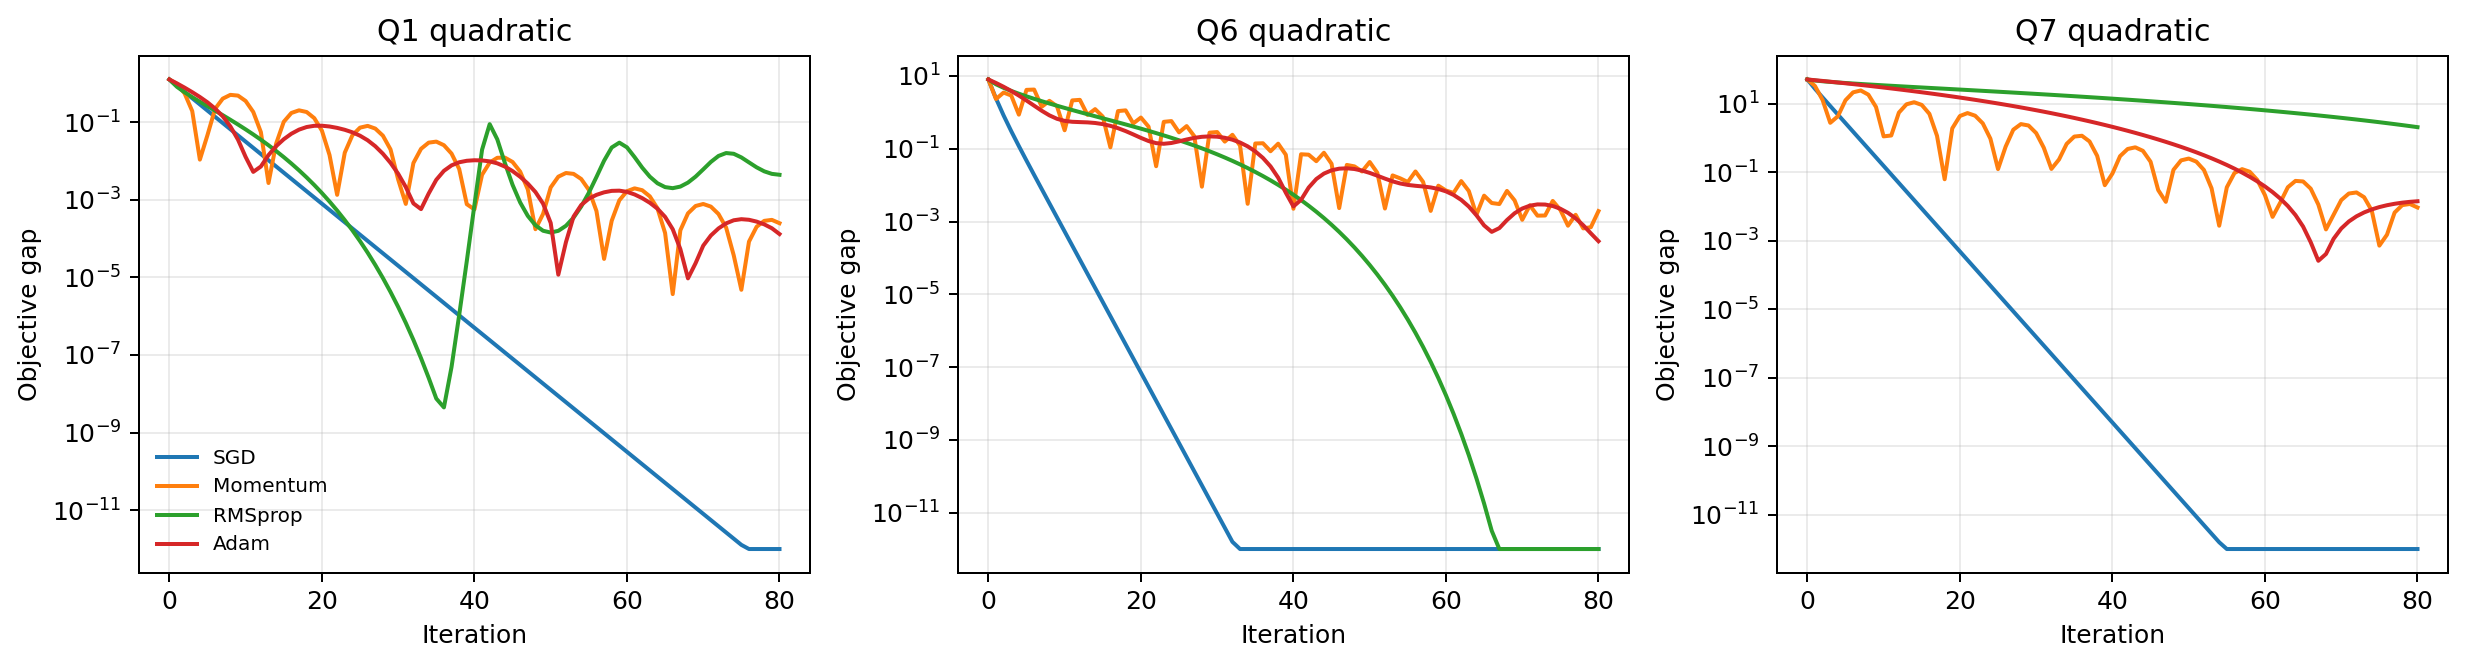
\includegraphics[width=0.92\textwidth]{q13_objective_gaps.png}
\caption{Q13：不同优化器在 Q1、Q6、Q7 上的目标值差距曲线}
\end{figure}

\begin{figure}[H]
\centering
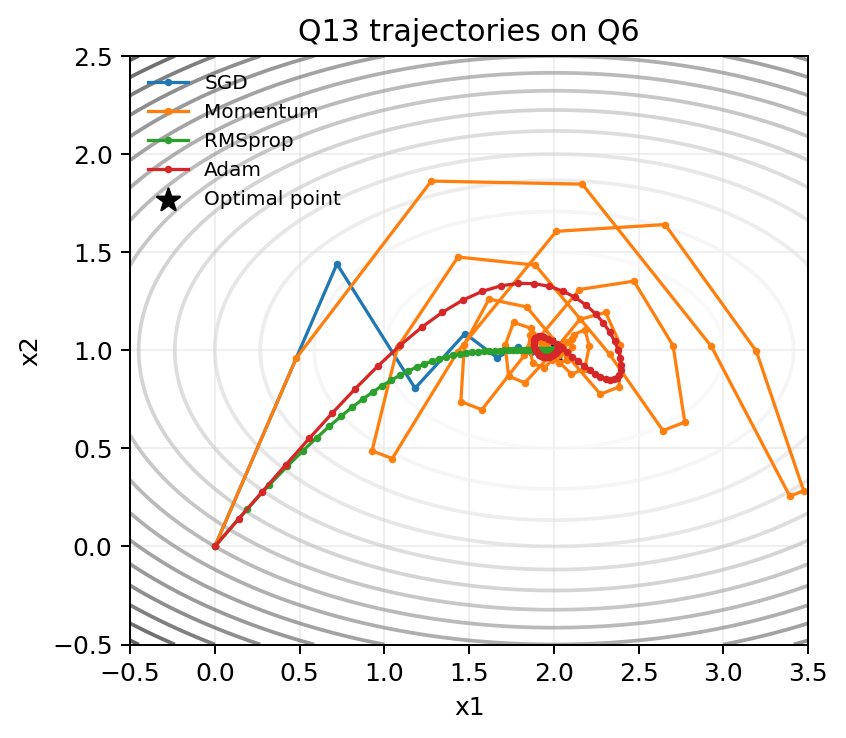
\includegraphics[width=0.62\textwidth]{q13_q6_trajectories.png}
\caption{Q13：不同优化器在 Q6 椭圆等高线上的轨迹}
\end{figure}

这些实验说明，深度学习一阶优化器的优势并不是“在所有简单凸问题上都必然优于 SGD”。在二维确定性二次问题上，若学习率已经手工调到很合适，普通 SGD 可以非常快地到达最优点；Momentum 和 Adam 由于引入了惯性或偏差校正，在短步数下反而可能出现过冲；RMSprop 对 Q6 这种坐标尺度不均匀的问题尤其有效，但对 Q7 的步长缩放并不理想。也就是说，深度学习优化器的价值主要体现在对尺度差异、噪声和复杂目标面的适应性上，而不是对所有低维凸问题的一刀切优势。

\subsection{题目九：随机初始化后的参数是否相似}

Q9 的核心问题是：两次随机初始化、长时间训练后的神经网络参数 $\theta_1$ 和 $\theta_2$ 是否相似。本文选取 Burgers PINN 中同一优化方法（Standard Adam）下的三次独立训练结果进行比较，得到如下数据：

\begin{table}[H]
\centering
\scriptsize
\resizebox{\textwidth}{!}{%
\begin{tabular}{llllrr}
\toprule
运行 A & 运行 B & 参数 $\ell_2$ 距离 & 参数余弦相似度 & 预测差异 MSE & 两次运行测试 MSE \\
\midrule
00\_24\_28 & 00\_35\_24 & 26.4920 & -0.00358 & $1.1418\times10^{-5}$ & $1.7298\times10^{-4}$ / $1.5222\times10^{-4}$ \\
00\_24\_28 & 00\_46\_10 & 26.0135 & 0.01701 & $1.3752\times10^{-5}$ & $1.7298\times10^{-4}$ / $1.7878\times10^{-4}$ \\
00\_35\_24 & 00\_46\_10 & 26.1322 & 0.01094 & $1.4350\times10^{-5}$ & $1.5222\times10^{-4}$ / $1.7878\times10^{-4}$ \\
\bottomrule
\end{tabular}
}
\caption{Q9：不同随机初始化的 Burgers PINN 最终参数比较}
\end{table}

该结果说明：在参数空间中，三次训练后的参数向量彼此相距很远，余弦相似度几乎为 0，甚至出现轻微负值，因此不能认为它们在参数空间中“相似”；但在函数空间中，三次训练得到的网络预测差异 MSE 只有 $10^{-5}$ 量级，而各自的测试误差都稳定在 $10^{-4}$ 量级，这说明它们实现了非常接近的输入输出映射。由此可以得到作业要求中的结论：\emph{随机初始化后的最终参数一般不相似，但对应函数往往相似。} 其根本原因在于神经网络目标函数高度非凸，且存在隐藏单元排列对称性和多模态低损失区域，因此“参数不同而功能接近”是常见现象。

\subsection{题目十四：训练参数是否服从低维特性}

Q14 使用现有 Burgers PINN 结果中的四类方法（standard、pcgrad、config、mconfig）、每类 3 个随机种子以及每次训练的 3 个时刻（epoch 0、15000、30000），总计 36 个参数快照。每个快照对应 10401 维参数向量。对这些参数向量做 PCA 后，前 8 个主成分的解释方差比如下：

\begin{table}[H]
\centering
\scriptsize
\begin{tabular}{lrrrr}
\toprule
主成分 & PC1 & PC2 & PC3 & 前三维累计 \\
\midrule
解释方差比 & 0.3234 & 0.3095 & 0.1399 & 0.7727 \\
\bottomrule
\end{tabular}
\caption{Q14：参数轨迹 PCA 的解释方差比}
\end{table}

\begin{figure}[H]
\centering
\begin{subfigure}{0.58\textwidth}
\centering
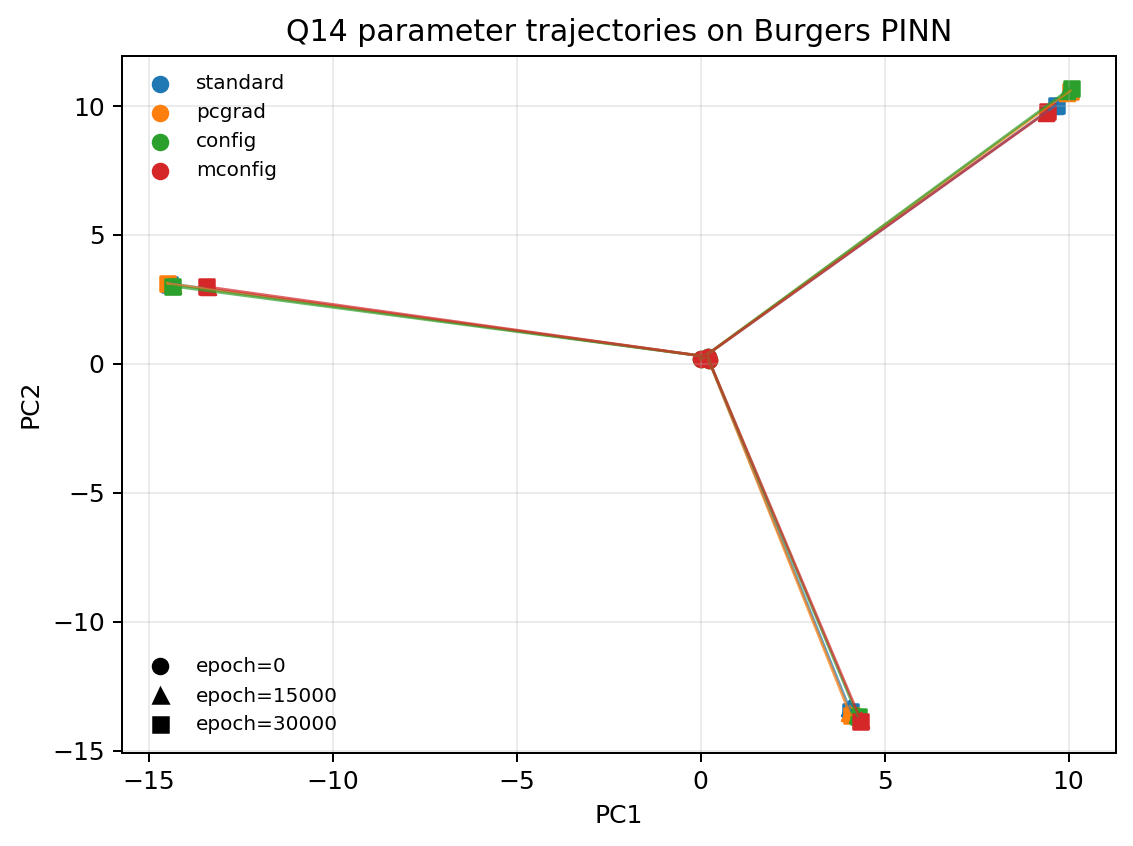
\includegraphics[width=\textwidth]{q14_parameter_trajectory_pca.png}
\caption{PC1--PC2 平面中的轨迹分布}
\end{subfigure}
\hfill
\begin{subfigure}{0.38\textwidth}
\centering
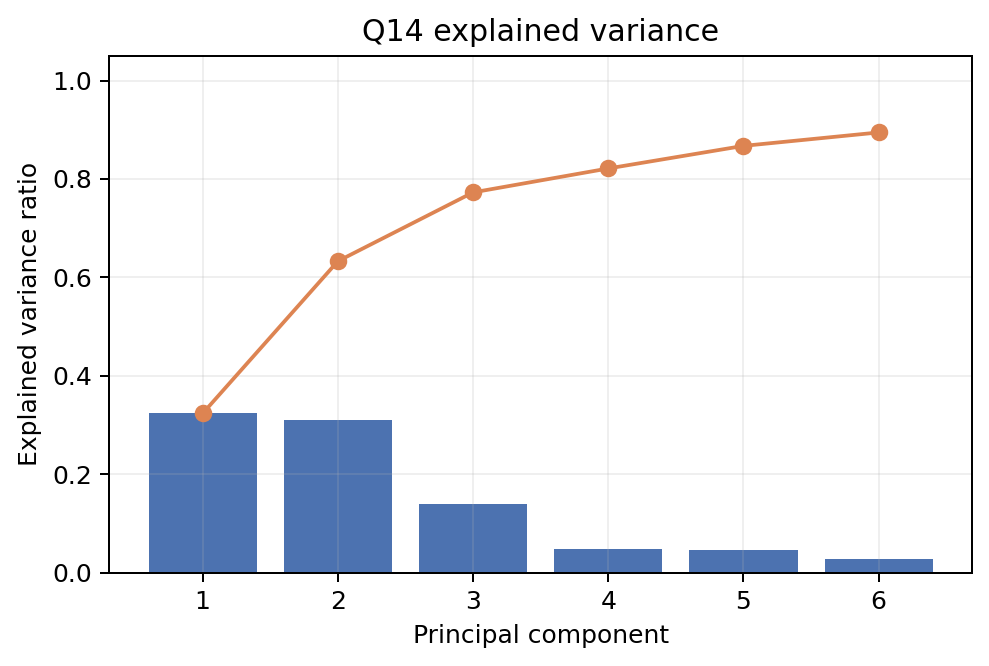
\includegraphics[width=\textwidth]{q14_explained_variance.png}
\caption{解释方差分布}
\end{subfigure}
\caption{Q14：Burgers PINN 参数轨迹的低维结构}
\end{figure}

图中可以看到，所有方法的初始点都聚集在原点附近，而训练后参数迅速沿若干主方向分叉，说明训练轨迹不是在高维空间中完全无规则地弥散，而是被少数主方向主导。从数值上看，前两个主成分已经解释了 63.29\% 的方差，前三个主成分解释了 77.27\% 的方差，因此“训练参数服从低维特性”这一判断得到了实证支持；但由于前两维尚未覆盖绝大部分方差，所以更准确的表述应是：\emph{Burgers PINN 的训练轨迹具有显著低维结构，但低维流形并非近似二维，而更接近三维及以上的低维子空间。}
同时也应看到，本文并没有记录每个 epoch 的连续轨迹，而是抽取了 epoch 0、15000、30000 三个代表时刻，因此这里验证的是“训练轨迹骨架”的低维性，而不是对全程连续流形的精细重建。如果后续将 checkpoint 频率进一步提高，那么可以更精确地区分“少数主方向主导”与“局部曲线弯折”这两种现象。

\section{理论推导与优化思想总结}

本节集中回答 Q4、Q8、Q10、Q11、Q12、Q15、Q17，对应作业中要求的理论证明与概念整理。

\subsection{题目四：次微分计算}

对凸函数 $f$，点 $x_0$ 处的次微分定义为
\[
\partial f(x_0)=\{g\in\mathbb{R}^n:\ f(x)\ge f(x_0)+g^T(x-x_0),\ \forall x\}.
\]

\paragraph{(a) $f(x_1,x_2,x_3)=\max\{|x_1|,|x_2|,|x_3|\}$ 在原点的次微分}
该函数就是 $\ell_\infty$ 范数，记为 $f(x)=\lVert x\rVert_\infty$。根据范数与对偶范数的标准结论，在原点处有
\[
\partial \lVert x\rVert_\infty\big|_{x=0}=\{g\in\mathbb{R}^3:\lVert g\rVert_1\le 1\}.
\]
因此
\[
\partial f(0,0,0)=\{g=(g_1,g_2,g_3)^T:\ |g_1|+|g_2|+|g_3|\le 1\}.
\]

\paragraph{(b) $f(x)=e^{|x|}$ 在 $x=0$ 的次微分}
记 $h(t)=e^t$、$g(x)=|x|$，则 $f(x)=h(g(x))$。因为 $h$ 在 $t=0$ 处可导且单调递增，所以由次微分链式法则可得
\[
\partial f(0)=h'(g(0))\,\partial g(0)=e^0\cdot[-1,1]=[-1,1].
\]

\paragraph{(c) $f(x_1,x_2)=\max\{x_1+x_2-1,\ x_1-x_2+1\}$ 在 $(1,1)$ 的次微分}
令
\[
g_1(x)=x_1+x_2-1,\qquad g_2(x)=x_1-x_2+1.
\]
在 $(1,1)$ 处有 $g_1(1,1)=g_2(1,1)=1$，因此两个分支同时激活。由最大值函数的次微分公式可得
\[
\partial f(1,1)=\mathrm{conv}\{\nabla g_1(1,1),\nabla g_2(1,1)\}
=\mathrm{conv}\{(1,1)^T,(1,-1)^T\}.
\]
故可写成参数形式
\[
\partial f(1,1)=\left\{\begin{pmatrix}1\\ 2\lambda-1\end{pmatrix}:\lambda\in[0,1]\right\}.
\]

\subsection{题目八：带噪声随机梯度的极限分布}

考虑迭代
\[
x_{t+1}=x_t-\lambda\bigl(\nabla f(x_t)+\sigma\xi_t\bigr),\qquad f(x)=\frac12\lVert x\rVert_2^2,
\]
其中 $\xi_t\sim N(0,1)$ 独立同分布。因为 $\nabla f(x_t)=x_t$，于是
\[
x_{t+1}=(1-\lambda)x_t-\lambda\sigma\xi_t.
\]
这是标准的一阶自回归过程。先看均值：
\[
\mathbb{E}[x_{t+1}]=(1-\lambda)\mathbb{E}[x_t].
\]
当 $0<\lambda<1$ 时，$|1-\lambda|<1$，因此 $\mathbb{E}[x_t]\to 0$。再看方差，利用 $x_t$ 与 $\xi_t$ 独立可得
\[
\mathrm{Var}(x_{t+1})=(1-\lambda)^2\mathrm{Var}(x_t)+\lambda^2\sigma^2.
\]
若极限方差记作 $V_\infty$，则它满足
\[
V_\infty=(1-\lambda)^2V_\infty+\lambda^2\sigma^2,
\]
从而
\[
V_\infty=\frac{\lambda^2\sigma^2}{1-(1-\lambda)^2}=\frac{\lambda^2\sigma^2}{2\lambda-\lambda^2}.
\]
因此当 $t\to\infty$ 时，$x_t$ 收敛到正态分布
\[
x_t\xrightarrow[]{d}N\left(0,\frac{\lambda^2\sigma^2}{2\lambda-\lambda^2}\right).
\]
噪声项 $\sigma\xi_t$ 的作用有两面性：一方面，它使得迭代无法精确停在最小值，而只能在最优点附近形成稳态分布；另一方面，在非凸问题中，这种随机扰动能够帮助算法逃离尖锐局部极小值和鞍点，因此常与更好的泛化表现联系在一起。

\subsection{题目十：梯度下降法与动量加速法的收敛性}

以下将“动量加速法”理解为 Nesterov 型加速梯度法。设 $f$ 是 $L$-smooth 凸函数，最优点为 $x^*$。

\paragraph{(a) 一般凸情形下的梯度下降}
取步长 $\alpha\le 1/L$，梯度下降迭代为
\[
x_{k+1}=x_k-\alpha\nabla f(x_k).
\]
由平方范数展开可得
\[
\lVert x_{k+1}-x^*\rVert^2
=\lVert x_k-x^*\rVert^2-2\alpha\nabla f(x_k)^T(x_k-x^*)+\alpha^2\lVert\nabla f(x_k)\rVert^2.
\]
因为 $f$ 是凸函数，
\[
f(x_k)-f(x^*)\le \nabla f(x_k)^T(x_k-x^*).
\]
又由于 $f$ 是 $L$-smooth 且 $\alpha\le 1/L$，有
\[
f(x_{k+1})\le f(x_k)-\frac{\alpha}{2}\lVert\nabla f(x_k)\rVert^2.
\]
将上述两个不等式合并，可得
\[
2\alpha\bigl(f(x_k)-f(x^*)\bigr)
\le \lVert x_k-x^*\rVert^2-\lVert x_{k+1}-x^*\rVert^2.
\]
对 $k=0,1,\ldots,N-1$ 求和可得
\[
f(x_N)-f(x^*)\le \frac{\lVert x_0-x^*\rVert^2}{2\alpha N},
\]
因此梯度下降在一般凸情形下具有 $O(1/N)$ 收敛率。

\paragraph{(b) 强凸情形下的梯度下降}
若进一步假设 $f$ 是 $\mu$-强凸函数，则有 Polyak--Łojasiewicz 型下界
\[
\lVert\nabla f(x)\rVert^2\ge 2\mu\bigl(f(x)-f(x^*)\bigr).
\]
配合 $\alpha=1/L$ 时的下降引理，得到
\[
f(x_{k+1})-f(x^*)
\le f(x_k)-f(x^*)-\frac{1}{2L}\lVert\nabla f(x_k)\rVert^2
\le \left(1-\frac{\mu}{L}\right)\bigl(f(x_k)-f(x^*)\bigr).
\]
递推可得
\[
f(x_k)-f(x^*)\le \left(1-\frac{\mu}{L}\right)^k\bigl(f(x_0)-f(x^*)\bigr),
\]
即线性收敛。

\paragraph{(c) Nesterov 动量加速}
Nesterov 加速梯度法可写为
\[
\begin{aligned}
y_k &= x_k+\beta_k(x_k-x_{k-1}),\\
x_{k+1} &= y_k-\frac1L\nabla f(y_k).
\end{aligned}
\]
其标准证明思路是构造估计序列或 Lyapunov 函数，并证明该势函数单调下降。由经典估计序列理论可得到：若 $f$ 是 $L$-smooth 凸函数，则
\[
f(x_k)-f(x^*)\le \frac{2L\lVert x_0-x^*\rVert^2}{(k+1)^2};
\]
若 $f$ 进一步是 $\mu$-强凸函数，令条件数 $\kappa=L/\mu$，则可以选取
\[
\beta=\frac{\sqrt{\kappa}-1}{\sqrt{\kappa}+1},
\]
并得到
\[
f(x_k)-f(x^*)\le C\left(1-\frac{1}{\sqrt{\kappa}}\right)^k.
\]
因此与普通梯度下降相比，动量加速法把一般凸情形的速率从 $O(1/k)$ 提升到 $O(1/k^2)$，并把强凸情形中的条件数依赖从 $\kappa$ 改善为 $\sqrt{\kappa}$。

\subsection{题目十一与十二：无约束优化思想、约束消除与变尺度法}

无约束优化的基本思想可以概括为三点：第一，利用梯度、Hessian 或近似 Hessian 构造下降方向；第二，通过线搜索或信赖域确定步长；第三，利用局部曲率信息改善条件数和收敛速度。将非凸问题转化为凸问题并不存在统一公式，但常见思路包括凸松弛、变量替换、提升到更高维的半正定松弛，以及对原问题做局部凸化。需要注意的是，这些转化通常只提供下界、近似解或局部有效的替代模型，并不保证与原问题完全等价。

有约束问题转化为无约束问题的常见手段则更为系统：罚函数法通过在目标函数中加入约束违反项，把约束“软化”为代价；障碍函数法通过在可行域边界附近引入发散项，保证迭代始终位于可行域内部；拉格朗日乘子法与增广拉格朗日法通过同时引入乘子和惩罚项，在数值上往往比单纯罚函数更稳定。实验二中使用的 ADMM，正是“有约束问题转为一系列无约束子问题”的典型例子。

从统一形式来看，最速下降法、牛顿法、修正牛顿法都可写为
\[
x_{k+1}=x_k+\alpha_k d_k,\qquad d_k=-B_k\nabla f(x_k),
\]
其中：
\[
B_k=I \Rightarrow \text{最速下降法},
\]
\[
B_k=[\nabla^2 f(x_k)]^{-1} \Rightarrow \text{牛顿法},
\]
\[
B_k=[\nabla^2 f(x_k)+\mu_k I]^{-1} \Rightarrow \text{修正牛顿法}.
\]
拟牛顿法或变尺度法的思想，就是不直接求真实 Hessian，而是迭代构造一个与 Hessian 逆矩阵具有相似作用的矩阵 $B_k$。几何上，它相当于不断重塑坐标系，使原本细长的椭圆等高线变得更接近圆形，从而减少最速下降法中的“之”字形震荡。

\subsection{题目十五：一阶优化算法的加速思想}

查阅 Lin 等人的教材与相关一阶优化文献后，可以把近年的加速思想概括为以下四类：

\begin{enumerate}
\item \textbf{外推与估计序列。} 这是 Nesterov 加速、FISTA 等方法的核心，通过在当前位置之外构造外推点来提高下降效率，本质上利用了“历史方向”来修正当前更新。
\item \textbf{复合优化中的近端加速。} 当目标函数包含光滑项和非光滑项时，近端映射允许把难处理的非光滑结构显式分离出来，再配合外推实现加速，例如 FISTA 和 Catalyst 框架。
\item \textbf{随机优化中的方差缩减。} SVRG、SAGA、Katyusha 等方法通过控制随机梯度的方差，使随机方法在保持较低单步成本的同时获得更快的全局收敛速度。
\item \textbf{自适应预条件与问题结构利用。} Adam、RMSprop 等方法通过对梯度做坐标尺度归一化改善病态问题；更一般地，K-FAC、Shampoo 等方法进一步尝试利用块结构或矩阵结构构造更强的预条件器。
\end{enumerate}

如果从“基本思想”而不是“算法名称”来总结，加速的一般规律可以表述为：\emph{要么利用历史信息构造更好的外推点，要么利用问题结构构造更好的度量，要么降低随机梯度噪声对迭代方向的破坏。} 这三类思想实际上贯穿了从 Nesterov 加速到现代自适应优化器的大部分发展路线。

\subsection{题目十七：共轭函数与对偶性的联系}

给定真值函数 $f: \mathbb{R}^n\to\mathbb{R}\cup\{+\infty\}$，其 Fenchel 共轭定义为
\[
f^*(y)=\sup_{x\in\mathrm{dom}(f)}\{y^Tx-f(x)\}.
\]
求共轭函数的过程，本质上是在所有 $x$ 中寻找使线性函数 $y^Tx$ 与原函数 $f(x)$ 之间差值最大的点。若 $f$ 可微且严格凸，则极值点满足
\[
y=\nabla f(x).
\]
例如，对于二次函数 $f(x)=\frac12\lVert x\rVert_2^2$，有
\[
f^*(y)=\frac12\lVert y\rVert_2^2.
\]
再如，若 $f=\delta_C$ 是集合 $C$ 的指示函数，则
\[
f^*(y)=\sup_{x\in C}y^Tx,
\]
即集合 $C$ 的支撑函数。

共轭函数与对偶性的联系在于：拉格朗日对偶中的“对原变量取下确界”常常等价于“对某个函数取共轭”。例如原问题
\[
\min_x f(x)\quad \text{s.t. } Ax=b
\]
的拉格朗日函数为
\[
L(x,\nu)=f(x)+\nu^T(Ax-b).
\]
对 $x$ 取下确界时，有
\[
\inf_x L(x,\nu)
=-b^T\nu+\inf_x\{f(x)+(A^T\nu)^Tx\}
=-b^T\nu-f^*(-A^T\nu).
\]
因此，对偶函数可以直接用共轭函数表示。也就是说，共轭函数不仅是一个定义，更是把原问题与对偶问题连接起来的关键桥梁。

\section{Krylov 子空间方法与 GMRES 数值示例}

本节对应 Q16。对于线性方程组 $Ax=b$，Krylov 子空间方法并不直接求 $A^{-1}$，而是在不断扩展的子空间
\[
\mathcal{K}_m(A,r_0)=\mathrm{span}\{r_0,Ar_0,A^2r_0,\ldots,A^{m-1}r_0\}
\]
中寻找近似解，其中 $r_0=b-Ax_0$ 是初始残差。这样做的优点是：在大规模稀疏问题中，只要能够快速完成矩阵向量乘法，就可以在不显式求逆的情况下逐步改进解。

GMRES 的目标是在当前 Krylov 子空间中选择一个向量，使残差范数最小；CG 则只适用于对称正定矩阵，并利用 $A$-共轭方向性质获得更低的存储和计算成本。为比较两者，本文构造了两个三对角矩阵：一个是对称正定矩阵，另一个是非对称矩阵。数值结果如下：
这里需要额外说明“迭代次数”的计数口径：CG 的迭代次数直接对应外层更新步数，而本文对 GMRES 记录的是回调函数被触发的内层残差更新次数，因此它更接近 Arnoldi 过程中的工作量统计，而不是 restart 轮数。换言之，表中 CG 与 GMRES 的迭代数可以用来反映数量级差异，但不应机械理解为完全同口径的一一对比。

\begin{table}[H]
\centering
\scriptsize
\begin{tabular}{llrrr}
\toprule
矩阵类型 & 方法 & 迭代次数 & 最终残差 & 解误差 \\
\midrule
对称正定三对角 & CG & 40 & 0 & $3.7570\times10^{-11}$ \\
对称正定三对角 & GMRES & 1424 & $9.9641\times10^{-11}$ & $5.6794\times10^{-7}$ \\
非对称三对角 & GMRES & 41 & $7.8945\times10^{-11}$ & $1.0678\times10^{-9}$ \\
\bottomrule
\end{tabular}
\caption{Q16：CG 与 GMRES 的数值比较}
\end{table}

\begin{figure}[H]
\centering
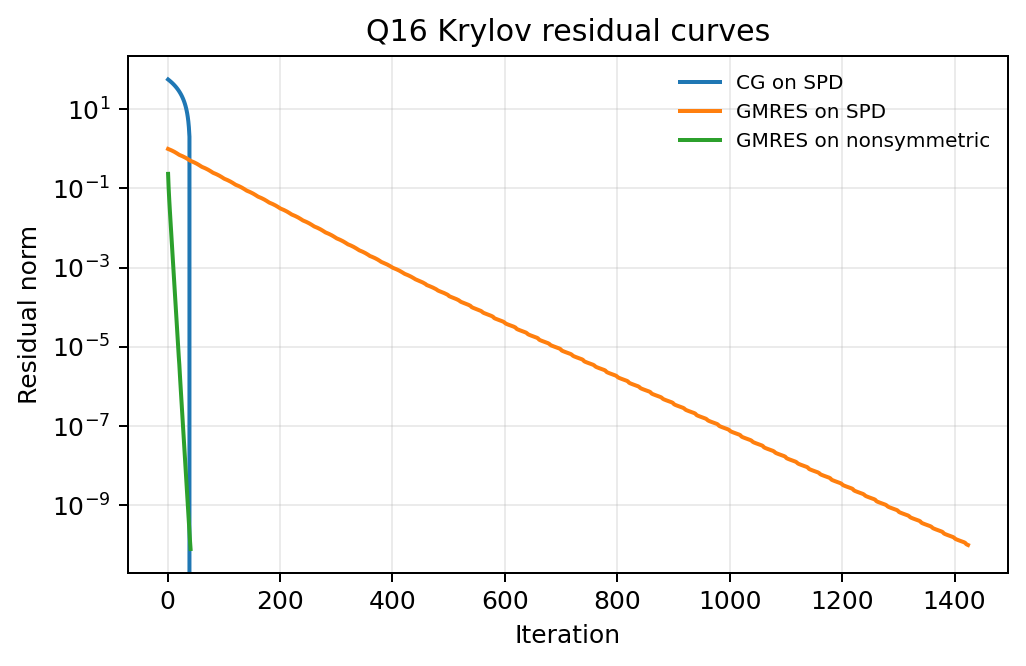
\includegraphics[width=0.72\textwidth]{q16_krylov_residuals.png}
\caption{Q16：Krylov 子空间方法的残差收敛曲线}
\end{figure}

这些结果说明：当矩阵是对称正定时，CG 利用了问题结构，明显快于 GMRES；但当矩阵变成非对称时，CG 不再适用，而 GMRES 仍能稳定求解。因此两者的根本差异不是“谁更快”，而是“谁利用了更多结构信息”。在适用条件满足时，CG 的内存和迭代成本更低；在一般非对称线性系统中，GMRES 的适用范围更广。

\section{结论}

通过本次作业，可以把课程中分散出现的若干概念重新串联起来。在线搜索层面，精确搜索与不精确搜索分别体现了“求最优步长”和“求可接受步长”两种思路；在方向更新层面，FR 共轭梯度、DFP 与 BFGS 展示了从一阶信息到近似二阶信息的不同利用方式；在理论层面，次微分、共轭函数、对偶性、带噪声 SGD 的极限分布等内容共同说明，现代优化并不只是算法堆叠，而是由几何、概率、凸分析和数值线性代数共同支撑的一套方法体系。

从扩展实验来看，深度学习优化器与传统数值优化器之间并不存在简单的“谁更先进”的关系。对于低维、结构明确且已经调好步长的二次问题，普通 SGD 仍然可以十分高效；而在真实神经网络训练中，参数空间的多模态与冗余结构更加突出，不同随机初始化可能对应完全不同的参数向量，却实现相近的函数行为。Burgers PINN 的 PCA 结果进一步说明，训练轨迹并非任意散布在高维空间中，而是被少数主方向控制，这为理解大规模神经网络训练的“低维有效自由度”提供了支持性证据。

\clearpage
\section*{参考文献}
\addcontentsline{toc}{section}{参考文献}

\begin{enumerate}[label={[\arabic*]}]
\item Yurii Nesterov. \emph{Introductory Lectures on Convex Optimization: A Basic Course}. Springer, 2004.
\item Zhouchen Lin, Risheng Liu, Huan Li. \emph{Accelerated Optimization for Machine Learning}. Springer, 2024.
\item Yousef Saad. \emph{Iterative Methods for Sparse Linear Systems}. SIAM, 2nd edition, 2003.
\item Timur Garipov, Pavel Izmailov, Dmitrii Podoprikhin, Dmitry Vetrov, Andrew Gordon Wilson. Loss Surfaces, Mode Connectivity, and Fast Ensembling of DNNs. NeurIPS, 2018.
\item Hao Li, Zheng Xu, Gavin Taylor, Christoph Studer, Tom Goldstein. Visualizing the Loss Landscape of Neural Nets. NeurIPS, 2018.
\item Xingchen Wan, Saining Xie, Kirill Brouzilis, et al. The Low-Dimensional Trajectory Hypothesis Is True: DNN Training Follows a Core Space. TPAMI, 2024.
\end{enumerate}

\appendix
\clearpage
\section{题号与实现位置对应表}

\begin{longtable}{>{\raggedright\arraybackslash}p{0.09\textwidth}>{\raggedright\arraybackslash}p{0.28\textwidth}>{\raggedright\arraybackslash}p{0.55\textwidth}}
\toprule
题号 & 报告位置 & 相关代码或资产 \\
\midrule
Q1 & 第 2 节第 3 小节 & \path{tools/Homework2/run_core_tasks.py} \\
Q2 & 第 2 节第 1 小节 & \path{tools/Homework2/src/line_search.py} \\
Q3 & 第 2 节第 2 小节 & \path{tools/Homework2/src/line_search.py} \\
Q4 & 第 4 节第 1 小节 & 本报告正文 \\
Q5 & 第 2 节第 3 小节 & \path{tools/Homework2/src/optimizers.py} \\
Q6 & 第 2 节第 3 小节 & \path{tools/Homework2/src/optimizers.py} \\
Q7 & 第 2 节第 3 小节 & \path{tools/Homework2/src/optimizers.py} \\
Q8 & 第 4 节第 2 小节 & 本报告正文 \\
Q9 & 第 3 节第 2 小节 & \path{tools/Homework2/run_report_tasks.py} \\
Q10 & 第 4 节第 3 小节 & 本报告正文 \\
Q11 & 第 4 节第 4 小节 & 本报告正文 \\
Q12 & 第 4 节第 4 小节 & 本报告正文 \\
Q13 & 第 3 节第 1 小节 & \path{tools/Homework2/src/dl_optimizers.py} \\
Q14 & 第 3 节第 3 小节 & \path{tools/Homework2/run_report_tasks.py} \\
Q15 & 第 4 节第 5 小节 & 本报告正文 \\
Q16 & 第 5 节 & \path{tools/Homework2/run_report_tasks.py} \\
Q17 & 第 4 节第 6 小节 & 本报告正文 \\
\bottomrule
\end{longtable}

\clearpage
\section{核心算法代码摘录}

为了让报告本身能够独立说明算法如何运行，本附录摘录了每类方法的核心实现。完整代码保存在附录 A 所列路径中，正文中的数值结果、表格和图形都由这些实现直接生成。

\subsection{精确一维搜索的统一调度接口}

下面代码展示了 Q2、Q5、Q6、Q7 中统一调用精确一维搜索的核心逻辑：先把多维目标限制到一条搜索直线，再根据方法名分派到二分法、黄金分割法、斐波那契法或 Shubert--Piyavskii 方法。

\begin{lstlisting}[language=Python, caption={精确一维搜索调度核心代码}]
def exact_search_along_direction(f, grad, x, direction, *, method="bisection", tol=1e-8):
    phi = lambda alpha: f(x + alpha * direction)
    phi_prime = lambda alpha: float(np.dot(grad(x + alpha * direction), direction))

    if method == "bisection":
        left, right = bracket_directional_derivative(phi_prime)
        return float(bisection_search(phi_prime, left, right, delta=tol, objective=phi)["x"])
    if method == "golden_section":
        left, right = bracket_minimum(phi)
        return float(golden_section_search(phi, left, right, tol=tol)["x"])
    if method == "fibonacci":
        left, right = bracket_minimum(phi)
        return float(fibonacci_search(phi, left, right, tol=tol)["x"])
    if method == "shubert_piyavskii":
        left, right = bracket_minimum(phi)
        sample_points = np.linspace(left, right, num=33)
        derivative_samples = [abs(phi_prime(point)) for point in sample_points]
        lipschitz = max(max(derivative_samples), 1.0)
        return float(shubert_piyavskii_search(phi, left, right, lipschitz=lipschitz, tol=tol)["x"])
\end{lstlisting}

\subsection{不精确一维搜索核心代码}

Q3 中实现了 Armijo、Goldstein、Wolfe--Powell 和强 Wolfe 规则。下面两段代码分别给出“充分下降”与“曲率条件”两类判据的核心实现。

\begin{lstlisting}[language=Python, caption={Armijo 线搜索核心代码}]
def armijo_search(f, grad, x, direction, *, alpha0=1.0, c1=1e-4, beta=0.5):
    phi, _phi_prime, phi0, phi_prime0 = _directional_setup(f, grad, x, direction)
    alpha = alpha0
    history = []

    while alpha > 1e-12:
        phi_alpha = phi(alpha)
        rhs = phi0 + c1 * alpha * phi_prime0
        accepted = phi_alpha <= rhs
        history.append({"alpha": alpha, "phi": phi_alpha, "rhs": rhs, "accepted": accepted})
        if accepted:
            return {"method": "armijo", "alpha": alpha, "phi": phi_alpha, "history": history}
        alpha *= beta
\end{lstlisting}

\begin{lstlisting}[language=Python, caption={Wolfe--Powell 线搜索核心代码}]
def wolfe_powell_search(f, grad, x, direction, *, alpha0=1.0, c1=1e-4, c2=0.9):
    phi, phi_prime, phi0, phi_prime0 = _directional_setup(f, grad, x, direction)
    alpha = alpha0
    lower, upper = 0.0, np.inf

    for _ in range(60):
        phi_alpha = phi(alpha)
        phi_prime_alpha = phi_prime(alpha)
        armijo_ok = phi_alpha <= phi0 + c1 * alpha * phi_prime0
        curvature_ok = phi_prime_alpha >= c2 * phi_prime0
        if armijo_ok and curvature_ok:
            return {"method": "wolfe_powell", "alpha": alpha, "phi": phi_alpha}
        if not armijo_ok:
            upper = alpha
            alpha = 0.5 * (lower + upper)
        else:
            lower = alpha
            alpha = 2.0 * alpha if np.isinf(upper) else 0.5 * (lower + upper)
\end{lstlisting}

\subsection{FR 共轭梯度法核心代码}

FR 共轭梯度法的关键在于用
\[
\beta_k=\frac{\lVert g_{k+1}\rVert_2^2}{\lVert g_k\rVert_2^2}
\]
更新搜索方向。对应实现如下：

\begin{lstlisting}[language=Python, caption={FR 共轭梯度法核心代码}]
def fr_conjugate_gradient(f, grad, x0, *, line_search, max_iter=200, tol=1e-6):
    x = np.asarray(x0, dtype=float).copy()
    g = grad(x)
    direction = -g

    for iteration in range(max_iter):
        if np.linalg.norm(g) < tol:
            break
        if float(np.dot(g, direction)) >= 0.0:
            direction = -g
        alpha = float(line_search(f, grad, x, direction))
        x_new = x + alpha * direction
        g_new = grad(x_new)
        beta = float(np.dot(g_new, g_new) / max(np.dot(g, g), 1e-30))
        direction = -g_new + beta * direction
        x, g = x_new, g_new
        if (iteration + 1) % x.size == 0:
            direction = -g
\end{lstlisting}

\subsection{DFP 与 BFGS 的逆 Hessian 更新}

Q5、Q6、Q7 中，DFP 与 BFGS 都维护 Hessian 逆矩阵的近似。它们的共同结构是：先根据当前近似矩阵计算方向，再通过 $s_k=x_{k+1}-x_k$ 与 $y_k=g_{k+1}-g_k$ 更新近似矩阵。

\begin{lstlisting}[language=Python, caption={DFP 更新核心代码}]
direction = -h_inv @ g
alpha = float(line_search(f, grad, x, direction))
s = alpha * direction
x_new = x + s
g_new = grad(x_new)
y = g_new - g
sy = float(np.dot(s, y))
hy = h_inv @ y
yhy = float(np.dot(y, hy))
if sy > 1e-12 and yhy > 1e-12:
    h_inv = h_inv + np.outer(s, s) / sy - np.outer(hy, hy) / yhy
\end{lstlisting}

\begin{lstlisting}[language=Python, caption={BFGS 更新核心代码}]
direction = -h_inv @ g
alpha = float(line_search(f, grad, x, direction))
s = alpha * direction
x_new = x + s
g_new = grad(x_new)
y = g_new - g
ys = float(np.dot(y, s))
if ys > 1e-12:
    rho = 1.0 / ys
    identity = np.eye(n)
    h_inv = (identity - rho * np.outer(s, y)) @ h_inv @ (identity - rho * np.outer(y, s)) + rho * np.outer(s, s)
\end{lstlisting}

\subsection{深度学习一阶优化器统一实现}

Q13 中的 SGD、Momentum、RMSprop 和 Adam 被写成统一接口，差异仅体现在更新规则上。这样既便于比较，也能保证实验入口一致。

\begin{lstlisting}[language=Python, caption={SGD、Momentum、RMSprop、Adam 的统一实现}]
def optimize(f, grad, x0, *, method, lr, steps, momentum=0.9, beta2=0.999, rho=0.9, eps=1e-8):
    x = np.asarray(x0, dtype=float).copy()
    velocity = np.zeros_like(x)
    sq_avg = np.zeros_like(x)
    first_moment = np.zeros_like(x)
    second_moment = np.zeros_like(x)

    for step in range(1, steps + 1):
        grad_vector = grad(x)
        if method == "SGD":
            update = grad_vector
        elif method == "Momentum":
            velocity = momentum * velocity + grad_vector
            update = velocity
        elif method == "RMSprop":
            sq_avg = rho * sq_avg + (1.0 - rho) * (grad_vector * grad_vector)
            update = grad_vector / (np.sqrt(sq_avg) + eps)
        elif method == "Adam":
            first_moment = momentum * first_moment + (1.0 - momentum) * grad_vector
            second_moment = beta2 * second_moment + (1.0 - beta2) * (grad_vector * grad_vector)
            first_hat = first_moment / (1.0 - momentum**step)
            second_hat = second_moment / (1.0 - beta2**step)
            update = first_hat / (np.sqrt(second_hat) + eps)
        x = x - lr * update
\end{lstlisting}

\subsection{Q16 中 CG 与 GMRES 的调用示例}

Q16 的重点不是手写完整 Krylov 求解器，而是给出一个可复现实验，展示 CG 与 GMRES 的适用范围与残差行为差异。下面是报告中实际使用的调用逻辑：

\begin{lstlisting}[language=Python, caption={CG 与 GMRES 的示例调用}]
spd_matrix = diags([-1.0, 2.0, -1.0], offsets=[-1, 0, 1], shape=(n, n), format="csr")
nonsym_matrix = diags([-1.0, 2.0, -0.5], offsets=[-1, 0, 1], shape=(n, n), format="csr")

x_cg, info_cg = cg(spd_matrix, b, rtol=1e-10, atol=0.0, maxiter=500, callback=cg_callback)
x_gmres_spd, info_gmres_spd = gmres(
    spd_matrix, b, rtol=1e-10, atol=0.0, restart=20, maxiter=500,
    callback=gmres_spd_callback, callback_type="pr_norm",
)
x_gmres_nonsym, info_gmres_nonsym = gmres(
    nonsym_matrix, b, rtol=1e-10, atol=0.0, restart=20, maxiter=500,
    callback=gmres_nonsym_callback, callback_type="pr_norm",
)
\end{lstlisting}

\end{document}